\chapter{Algerian Arabic Corpus by Data Augmentation}
\pagestyle{fancy}\lhead{\textbf \footnotesize\it{Algerian Arabic Corpus by Data Augmentation}}
\pagestyle{fancy}\chead{} \pagestyle{fancy}\rhead{}
\pagestyle{fancy}\lfoot{\textbf {\small\it{Univ-Mascara/Computer Science: 2024}}} 
\pagestyle{fancy}\cfoot{} \pagestyle{fancy}\rfoot{\thepage}
%%%%%%%%%%%%%%%%%%%%%%%%%%%%%%%%%%%%%%%%
\section{Overview}\label{start5}
In this chapter, we delve into the vital significance of corpora and data augmentation techniques in bolstering machine translation (MT) systems. 
We commence by detailing the essence of both monolingual and bilingual corpora, elucidating existing data sources in the process. 
Furthermore, we underscore the critical role of data preprocessing, delving into methodologies aimed at refining corpora to uphold quality and ensure consistency throughout the dataset.

We then delve into monolingual corpora augmentation methods, including copied-corpus augmentation (CC) and back-translation augmentation (BT), which leverage additional data to enhance model performance. 
Furthermore, we introduce two novel augmentation strategies tailored to Arabic languages: Right Rotation Augmentation (RRA) and Entity Replacement Augmentation (ERA). 
These approaches aim to address challenges in low-resource language translation by diversifying datasets and incorporating culturally relevant substitutions. 
Throughout, we underscore the critical role of effective data preprocessing and augmentation in optimizing MT systems for improved translation accuracy and linguistic understanding.

\section{Bilingual Corpora}\label{start5.1}
Corpus-based approaches to MT, like Statistical Machine Translation (SMT) and Neural Machine Translation (NMT), emerged with the growing availability of parallel corpora or bitexts, which consist of texts translated into different languages. 
These methods capitalize on the translations created by human translators, utilizing them within machine learning frameworks to construct translation models. 
High-quality and substantial amounts of parallel data are crucial for training optimal models, as highlighted by \cite{koehn17, lample18}. 
Unlike English, the main issue that faces the Arabic language is the lack of sufficient available datasets; particularly, the parallel datasets; which makes Arabic and dialectal Arabic considered low resource languages (LRLs). The disparities between what can be categorized as high, medium, and low resource language pairs are shown in Table~\ref{tab:LRL} \cite{haddow22}.
Consequently, a significant challenge in translating low-resource languages lies in obtaining sufficiently large and clean parallel corpora.
\begin{table}[]
	\centering
	\begin{tabular}{ l l r } 
		\hline
		Resource Level & Language Pair & Parallel Sentences \\
		\hline
		High & English–French & 280M \\
		Medium & English–Myanmar & 0.7M \\ 
		Low & English–Fon & 0.035M \\ 
		\hline
	\end{tabular}
	\caption{Examples of language pairs with different levels of resources.}
	\label{tab:LRL}
\end{table}

DZDA (Algerian Dialectal Arabic) serves as another example of a low-resource language explored in this research. 
DZDA, a variant of Arabic predominantly spoken in Algeria, is heavily influenced by various linguistic sources, including French, Spanish, and Berber. 
This linguistic diversity poses challenges for Natural Language Processing (NLP) tasks due to the scarcity of tools and resources tailored to this specific dialect \cite{samih17}. 
Moreover, in media content, written texts in DZDA may feature a mix of Arabic script, Latin script, and transliterated words to Latin. 
This complexity in script and vocabulary adds to the difficulty of processing and analyzing DZDA text, especially in the context of social media content where linguistic variations and informal expressions are prevalent.

The existing corpora (Section~\ref{start5.2}) for DZDA are either limited in size or suffer from poor quality; they are predominantly sourced from online platforms, including crowd translation efforts. 
Relying on the internet as a corpus repository is driven by the desire to access extensive data at minimal cost. 
However, these sources often lack consistency and may contain inaccuracies, posing challenges for machine translation. 
Moreover, given the absence of standardization in DZDA, variations in language usage and style are common across different sources. 
As a result, manual or automated methods for data cleaning and alignment are necessary to address these issues and improve the quality of MT outputs.

\section{Monollingual Corpora}
Statistical Machine Translation (SMT) relies on monolingual corpora to develop language models. 
Although not mandatory for Neural Machine Translation (NMT), monolingual corpora can aid in generating synthetic parallel sentences through techniques like back-translation (BT), where monolingual data in the target language is utilized, and forward-translation (FT), where the monolingual corpus is in the source language.

\section{Existing Corpora}\label{start5.2}
There are two free datasets available for the task of machine translation between Algerian Arabic dialect and Modern Standard Arabic (MSA): PADIC\footnote{PADIC dataset is available at: https://sourceforge.net/projects/padic/} (Parallel Arabic Dialect Corpus) \cite{meftouh15}, MADAR\footnote{MADAR dataset is available at: https://github.com/farahshamout/madar-dataset} (Multi Arabic Dialect Applications and Resources) \cite{bouamor18}, and ANMaT, our in-house dataset\footnote{an internally created dataset is available at: https://github.com/bbaligh/DZDA-MSA/}.
Table~\ref{tab:bi-datasets} summarizes the statistics for each dataset, encompassing metrics such as the quantity of parallel sentences, overall word count, vocabulary size, and average sentence length.

\section{Data Sources}
PADIC encompasses a collection of five dialects: one from Syria, one from Tunisia, one from Palestine, and two originating from Algeria (\textbf{Algiers}, \textbf{Annaba}), constituting a total of 6,400 parallel sentences for each dialect.
The MADAR dataset comprises 25 Arabic dialects, featuring cities such as Beirut, Cairo, Doha, Rabat, Tunis, Aleppo, Alexandria, \textbf{Algiers}, Amman, Aswan, Baghdad, Basra, Benghazi, Damascus, Fes, Jeddah, Jerusalem, Khartoum, Mosul, Muscat, Riyadh, Salt, Sanaa, Sfax, and Tripoli, each containing 2,000 sentences. 
Thus, the total size of MADAR amounts to 50,000 sentences.

ANMaT, the in-house dataset, was created for the purpose of enhancing MT efforts, was meticulously assembled by two expert native speakers fluent in both the Algerian Arabic Dialect (DZDA) and Modern Standard Arabic (MSA). 
Using a specialized web scraping tool, a rich array of bilingual sentence pairs was compiled from diverse social media sources, such as Twitter, YouTube, and Facebook. 
Adhering to a strict one-to-one correspondence, each sentence from one language was carefully translated to the other, with thorough preprocessing to guarantee the uniformity and quality of the data. 
The engagement of two native speakers contributed to the dataset's linguistic accuracy, enriching it with cultural nuances and idiomatic phrases unique to the Algerian Arabic Dialect and Modern Standard Arabic. 
To protect user privacy, anonymization measures were taken, ensuring the in-house dataset's data remained confidential and secure throughout the translation effort. 
The collection consists of around 1,800 sentence pairs, featuring parallel texts in DZDA and MSA.

\begin{table}[htbp]%[htb]
	\centering
	%	\begin{center}
		%		\begin{minipage}{\textwidth}%{280pt}
			\begin{tabular}{llcccc}
				\hline
				\multirow{2}{*}{Dataset} & \multirow{2}{*}{Language} & \# & \multirow{2}{*}{Vocabulary} & \# & Average\\
				&  & Tokens & & Sentences & length\\
				\hline
				\multirow{2}{*}{PADIC} & MSA  & 87,680 & 8,374 & \multirow{2}{*}{6,412} & 13.65\\
				& DZDA & 78,614 & 7,613 &  & 12.26\\
				\hline
				\multirow{2}{*}{MADAR} & MSA  & 15,929 & 4,408 & \multirow{2}{*}{2,000} & 10.23\\
				& DZDA & 13,198 & 4,180 &  & 8.56\\
				\hline
				\multirow{2}{*}{ANMaT} & MSA  & 17,594 & 2,632 & \multirow{2}{*}{1,800} & 12.09\\
				& DZDA & 17,877 & 3,200 &  & 12.23\\
				\hline
				\multirow{2}{*}{Consolidated Dataset} & MSA  & 132,512 & 11,492 & \multirow{2}{*}{10,212} & 14.04\\
				& DZDA & 119,664 & 11,927 &  & 12.71\\
				\hline
			\end{tabular}
			%		\end{minipage}
		%	\end{center}
	\caption{Statistic of the MSA$\leftrightarrow$DZDA corpora}
	\label{tab:bi-datasets}
\end{table}

\section{Preprocessing}
The dataset pre-processing steps outlined in the algorithm~\ref{algo:Algo1} encompass a series of cleaning and selecting procedures to prepare the data for further analysis. 
Initially, the cleaning phase involves the removal of non-alphanumeric characters from the dataset to ensure data cleanliness. 
Subsequently, sentences exhibiting a length ratio greater than 3 or less than 0.3 are eliminated, as they are considered outliers in terms of length discrepancy. 
Additionally, sentences with a lexical overlap of less than 0.5 are removed to enhance the dataset's lexical consistency. 
%Following the cleaning process, the dataset undergoes a splitting phase, where it is divided into three distinct sets. 
%Specifically, 80\% of the dataset is randomly selected to form the training set. 
%From the remaining data, 10\% is randomly chosen to create the validation set. 
%The test set is then composed of the residual data, excluding the previously selected training and validation sets. 
%This systematic approach ensures a structured division of the dataset into training, validation, and test sets, facilitating comprehensive evaluation and training of models on cleansed and well-distributed data.

\begin{algorithm}
	\begin{algorithmic}[1]
		\caption{Dataset pre-processing steps}
	\label{algo:Algo1}
		\State /* Dataset cleaning */
		\State Remove non-alphanumeric characters 
		\State Remove sentences with a length ratio $> 3$ or $< 0.3$
		\State Remove sentences with a lexical overlap $< 0.5$
%		\State /* Dataset split */ 
%		\State Training\_set $\leftarrow$ RandomSelection(Dataset, 80\%)
%		\State Validation\_set $\leftarrow$ RandomSelection(Dataset$-$Training\_set, 10\%)
%		\State Test\_set $\leftarrow$ Dataset$-$Training\_set$-$Validation\_set
	\end{algorithmic}
\end{algorithm}
	
%\section{Monollingual Corpora}
%SMT requires monolingual corpora to generate a language model. 
%While not essential for NMT, monolingual corpora can facilitate the creation of artificial parallel sentences through back-translation (BT). 
%Moreover, data-driven methods for spelling correction also necessitate monolingual corpora.

%\subsection{Existing Monolingual Corpora}
%
%\subsection{Data Sources}
%
%\subsection{Preprocessing}

\section{Data Augmentation}
NMT is extremely data-hungry \cite{sutskever14, bahdanau15, vaswani17} and the presence of abundant, high-quality parallel data is essential for achieving the best outcomes.  
So, when working with LRLs, it is critical to employ approaches that increase corpora size in order to attain better MT quality.
There are numerous approaches to increasing the size of the corpora and improving model performance such as: backward translation (henceforth BT) \cite{sennrich16, edunov18} which is an approach where a backward model is used to generate hypotheses of the source language in order to increase the amount of data available to translation systems, forward translation (henceforth FT) \cite{zhang20} which works in the opposite direction, employing a forward model to predict translations in the target language - a process known as Self-learning., and the copied-corpus approach, in which target sentences are copied on the source side \cite{ha16} (called Mix-source) or, inversely, by making a copy of source sentences into the target side \cite{sanchez21}. 
Recent research has shown that different approaches, including back-translation, sub-word units, and adapting NMT systems to low-resource settings \cite{sennrich19}, can improve NMT performance with low-resource scenarios.
\subsection{Monolingual corpora Augmentation}

\subsubsection{Copied-corpus Augmentation}
This method enhances training datasets by copying existing sentences from the target language to the source language (termed Mix-source) or the other way around.
Originally inspired by self-teaching strategies in MT, the approach was first introduced by \cite{ha16}, who proposed the Mix-source method of duplicating target language sentences on the source side (see Figure~\ref{fig:cc}). 
Following this, \cite{sanchez21} explored the inverse, where source language sentences are replicated on the target side. 
This straightforward method boosts the available training material by reusing the corpus in new ways, broadening the model's exposure to different translation possibilities and linguistic patterns. 
Such exposure can significantly enrich the model's performance across various MT tasks.

\begin{figure}[H]
	\centering
	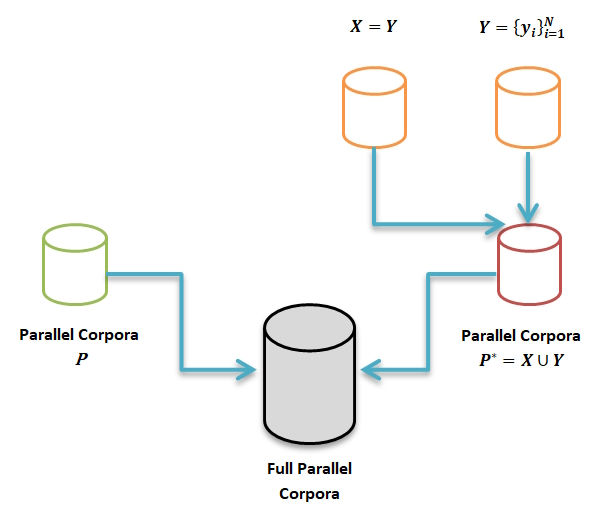
\includegraphics[width=0.6\linewidth]{Figures/CC}
	\caption{The copied-corpus augmentation approach}
	\label{fig:cc}
\end{figure}

The advantages of copied corpus augmentation extend beyond simply enlarging the dataset. 
It notably addresses the challenge of limited data resources, a frequent obstacle in MT, especially with under-represented languages. 
By multiplying the available examples, it enables the model to better generalize from its training, enhancing its capability to deal with novel vocabulary or sentence structures. 
This method is especially relevant for neural machine translation systems that thrive on recognizing data patterns. 
Replicating sentences across language boundaries may reinforce pattern recognition, thereby increasing translation precision.

Nevertheless, this technique is not without its potential downsides. 
The act of copying sentences might not always yield semantically rich training examples, requiring careful strategy selection to avoid injecting noise into the dataset. 
Furthermore, its efficacy can fluctuate based on the specific language combination and the architecture of the MT system being used.
Despite these considerations, copied corpus augmentation stands as a notably straightforward yet potent strategy for enhancing data volume in machine translation. 
Its capacity to mitigate data scarcity issues and boost model performance renders it an invaluable asset for MT researchers and developers.

\subsubsection{Back Translation Augmentation}
Enhancing Neural Machine Translation (NMT) quality can be achieved by leveraging extra monolingical resources to generate synthetic training data. 
Typically, monolingual data on the source side is translated into the target language (FT), while target-side monolingual data undergoes back BT. 
This synthetic data is then incorporated with the initial bilingual corpus. 

BT involves translating sentences from a target language back into the source language using an existing NMT model. 
These back-translated sentences are then paired with their original target language sentences, effectively creating new, synthetic source-target sentence pairs (see Figure~\ref{fig:bt}). 
This method significantly enriches the training dataset, especially with examples that might not be present in the original parallel corpus. 
By leveraging monolingual data in the target language, back translation helps in bridging the gap in data scarcity and improves the NMT model's ability to understand and translate nuanced and complex sentence structures. 
This technique has been widely acknowledged for its capacity to boost the quality of machine translations, making it a favored choice among researchers and practitioners aiming to enhance the performance of MT systems, particularly in scenarios involving low-resource languages.
It's commonly acknowledged that BT significantly enhances Neural Machine Translation more effectively than FT \cite{bogoychev19}.

\begin{figure}[ht]
	\centering
	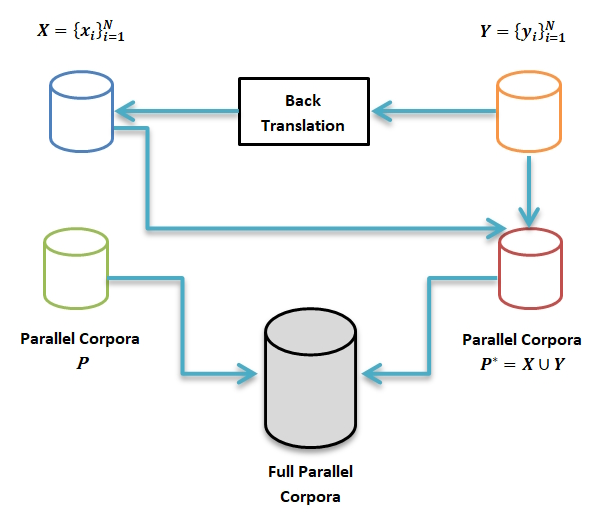
\includegraphics[width=0.6\linewidth]{Figures/BT}
	\caption{The back-translation augmentation approach}
	\label{fig:bt}
\end{figure}

\subsection{Parallel Corpora Augmentaiton}
\subsubsection{Right Rotation Augmentation}
After exploring monolingual augmentation strategies such as copied-corpus augmentation and back-translation, we now introduce a novel method tailored to the unique syntactic properties of Arabic and implemented on bilingual corpora, dubbed "Right Rotation Augmentation". 
This technique leverages the flexible word order in Arabic sentence construction, where, due to its non-configurational nature, elements within a sentence can often be rearranged without altering the sentence's meaning. 

\begin{figure}[h]
	\centering
	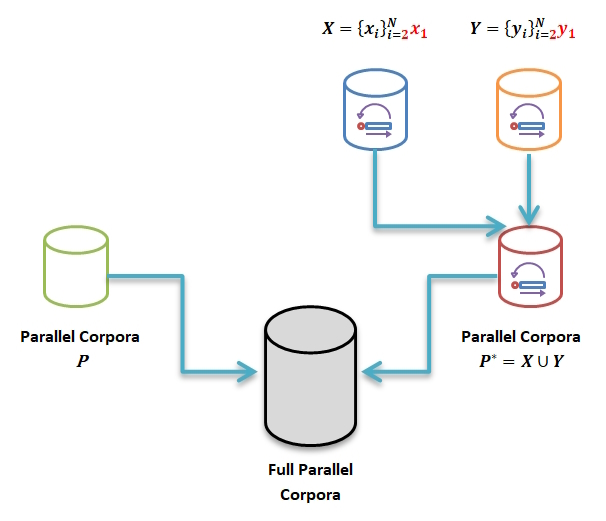
\includegraphics[width=0.6\linewidth]{Figures/RRA}
	\caption{The Right-rotation augmentation approach}
	\label{fig:rra}
\end{figure}

Right Rotation Augmentation systematically rotates the sentence structure to the right, creating multiple valid syntactic variations of the same sentence. 
For instance, a sentence beginning with a verb can be transformed to start with its object or subject without losing coherence (see Figure~\ref{fig:rra}). 
This method not only enriches the dataset with diverse syntactic representations but also helps machine translation models better grasp the variability and richness of Arabic syntax. 
By incorporating such rotated sentences into the training data, models can learn to recognize and translate a wider array of sentence constructions, potentially improving translation accuracy and robustness, especially for languages with free or flexible word order like Arabic.

The Right Rotation Augmentation (RRA) algorithm (see Algorithm~\ref{algo:rra}) takes a sentence pair as input and applies right rotation to both the source and target sentences, generating four augmented sentence pairs with varied word orders. 
This approach introduces diversity into the training data, potentially enhancing the robustness and performance of machine translation models.
The new size of the resulting augmented dataset using RRA is four times the original size of the dataset.

\begin{algorithm}[H]
	\caption{Right Rotation Augmentation (RRA)}
	\label{algo:rra}
	\KwIn{A sentence pair $S_1$-$T_1$ (where $S_1$ represents the source sentence and $T_1$ denotes the target sentence)}
	\KwOut{Four augmented sentence pairs: $S_1$-$T_1$, $S'_1$-$T_1$, $S_1$-$T'_1$, and $S'_1$-$T'_1$}
	\BlankLine
	/* Apply Right Rotation to $S_1$ \;
	$S'_1 \leftarrow$ Rotate the source sentence $S_1$ by moving the first word to the end\;
	/* Apply Right Rotation to $T_1$ \;
	$T'_1 \leftarrow$ Rotate the target sentence $T_1$ by moving the first word to the end\;
	\Return{Original sentence pair $S_1$-$T_1$, Augmented pair $S'_1$-$T_1$, Augmented pair $S_1$-$T'_1$, Augmented pair $S'_1$-$T'_1$}
\end{algorithm}


\subsubsection{Entity Replacement Augmentation}
A novel augmentation method, termed Entity Replacement Augmentation (ERA) or Lexicon-based Entity Substitution Augmentation, has been created specifically for low-resource languages, including Algerian Dialectal Arabic (DZDA) and Modern Standard Arabic (MSA) in our case.
This method involves substituting entities, such as person or location names, using a predefined lexicon. 
By replacing these entities with alternate names from the lexicon, fresh sentences can be generated while preserving the original sentences' structure and context. 
This method aims to enrich the dataset by introducing variations in the mentioned names, potentially enhancing the model's capacity to handle diverse linguistic scenarios. 
Moreover, by integrating culturally relevant names into the augmented dataset, the approach seeks to enhance the model's grasp of context-specific language usage, thereby contributing to more precise and culturally attuned translations.

To execute this task, first, we need to compile a lexicon containing alternative names for entities commonly found in the text, such as names of people, places, organizations, and other relevant entities. 
This lexicon can be sourced from various resources, including dictionaries, databases, or even generated using statistical methods based on the existing dataset. 
Once the lexicon is prepared, we identify the entities within the sentences that we intend to augment. 
For each identified entity, we randomly select a replacement name from the lexicon. 
Finally, we substitute the original entity with the chosen replacement name, generating new sentences with the altered entities. 
This process is repeated iteratively for multiple sentences in the dataset, resulting in an augmented dataset with variations in entity names.

\begin{algorithm}[H]
	\SetAlgoLined
	\KwIn{Sentence pairs \( S1-T1 \) (S1: source sentence, T1: target sentence), Lexicon containing alternative names for entities}
	\KwOut{Augmented sentence pairs}
	\SetKwInOut{Input}{Input}
	\SetKwInOut{Output}{Output}
	\Input{Sentence pairs \( S1-T1 \) (S1: source sentence, T1: target sentence), Lexicon containing alternative names for entities}
	\Output{Augmented sentence pairs}
	\BlankLine
	\For{each sentence pair \( (S1, T1) \) in the dataset}{
		Identify entities in \( S1 \) and \( T1 \)\;
		\For{each identified entity in \( S1 \)}{
			Select a random replacement name from the lexicon\;
			Replace the entity in \( S1 \) with the chosen replacement name\;
		}
		\For{each identified entity in \( T1 \)}{
			Select a random replacement name from the lexicon\;
			Replace the entity in \( T1 \) with the chosen replacement name\;
		}
		Append the original sentence pair \( (S1, T1) \) and the modified pair \( (S'1, T'1) \) to the augmented dataset\;
	}
	\caption{Entity Replacement Augmentation}
\end{algorithm}

\section{Summary}
In conclusion, this chapter has explored various strategies aimed at optimizing machine translation (MT) through the utilization of different types of corpora and data augmentation techniques. 
We began by highlighting the significance of monolingual and bilingual corpora as essential resources for MT tasks, emphasizing their role in training robust models. 
Subsequently, we delved into the preprocessing steps necessary for refining corpora to ensure data quality and consistency, emphasizing the importance of thorough cleaning and normalization procedures. 

Furthermore, we investigated monolingual corpora augmentation methods, focusing on copied-corpus (CC) and back-translation (BT) techniques, which leverage additional monolingual data to augment training sets and improve model performance. 
Additionally, we introduced two novel augmentation approaches tailored to Arabic languages: Right Rotation Augmentation (RRA) and Entity Replacement Augmentation (ERA). 
RRA involves rotating sentence structures to diversify datasets, while ERA substitutes entities like names with culturally relevant alternatives, enriching training data. 
These strategies aim to address challenges posed by low-resource languages and enhance translation accuracy. 
Throughout the chapter, we emphasized the significance of effective data preprocessing and augmentation in optimizing MT systems for improved linguistic understanding and translation capabilities.








%In the pursuit of enhancing machine translation performance, various augmentation techniques have been explored, catering to both monolingual and bilingual corpora. 
%
%Monolingual corpora augmentation strategies, such as copied-corpus and back-translation, involve leveraging existing data within a single language to create synthetic training examples or translate source data into the target language, respectively. 
%
%On the other hand, bilingual corpora augmentation methods, including Right Rotation Augmentation (RRA) and Entity Replacement Augmentation (ERA), target the enhancement of bilingual datasets. 
%RRA introduces variations in sentence structure by rotating words within sentence pairs, while ERA focuses on replacing entities like names or locations with alternatives from a predefined lexicon. 
%
%These augmentation approaches collectively aim to diversify datasets, improve model generalization, and enhance translation quality across low-resource languages, exemplifying innovative strategies in the field of machine translation augmentation.

